% ICLR 2027 single-column figures. Requires graphicx.
\begin{figure}[t]
    \centering
    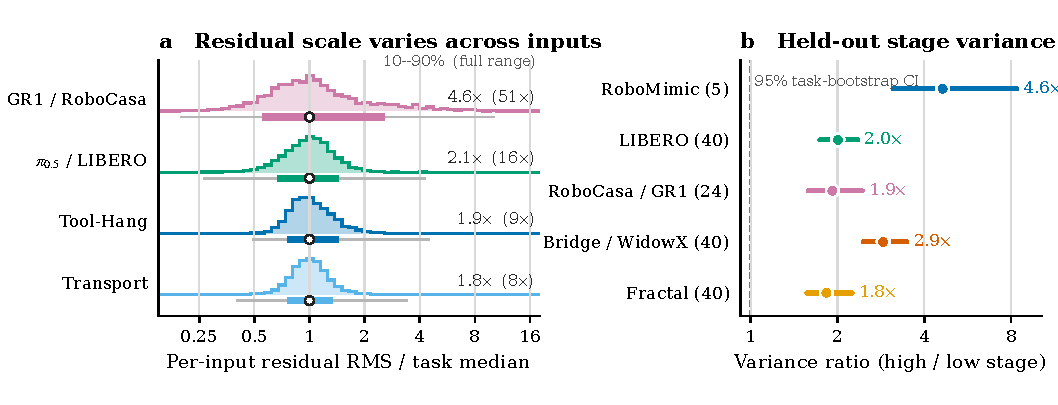
\includegraphics[width=\linewidth]{analysis/paper/data_ht_motivation/fig_crossdataset_stage_scale.pdf}
    \caption{\textbf{Action residuals require input-dependent variance.}
    \textbf{Left:} using frozen MSE policies as conditional-mean estimators, we
    plot the per-input RMS of eight-step continuous-action residuals, normalized
    by the median within each task. The frozen MSE policies are GR00T N1.7 on
    GR1/RoboCasa, $\pi_{0.5}$ on LIBERO, and Chi-UNet on RoboMimic. Thick bars and the first number report the
    10th--90th-percentile span; thin bars and parenthesized numbers report the
    full observed range. On GR1/RoboCasa, for example, the central 80\% spans
    $4.6\times$ and the full range spans $51\times$.
    \textbf{Right:} a data-only cross-demonstration test verifies that this is
    not merely MSE fitting error. For every task stage, we estimate an action
    radius from one demonstration fold, rank stages by that radius, and measure
    residual variance on disjoint demonstrations. High-radius stages exhibit
    $1.8$--$4.6\times$ the held-out variance of low-radius stages across all five
    datasets; intervals are 95\% task-bootstrap CIs. The analysis covers 149
    tasks and 3,688 demonstrations. Binary grippers are excluded; continuous GR1
    hand joints are retained.}
    \label{fig:data-phase-scale}
\end{figure}

\begin{figure}[t]
    \centering
    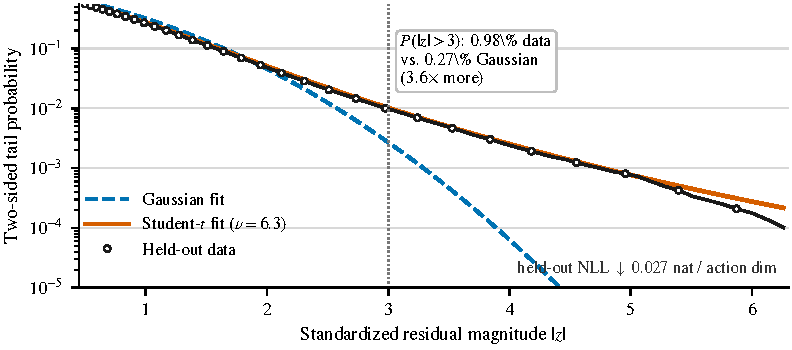
\includegraphics[width=\linewidth]{analysis/paper/data_ht_motivation/fig_heavy_tailed_residuals.pdf}
    \caption{\textbf{Locally standardized continuous-action residuals remain
    heavy-tailed.} We first divide each residual by its state-local RMS and
    then normalize every chunk coordinate by its training-fold RMS, removing
    phase-level and coordinate-level scale differences. Curves are evaluated
    on disjoint held-out demonstrations. The empirical probability beyond
    $3$ standard deviations is 0.98\%, compared with 0.27\% under the fitted
    Gaussian. A Student-$t$ fit ($\nu=6.3$) follows the empirical tail and
    reduces held-out negative log-likelihood by 0.027 nat per action
    dimension. The binary gripper channel is excluded.}
    \label{fig:data-heavy-tail}
\end{figure}
